\documentclass{article}
\usepackage{tikz, comment}
\usepackage{pifont}
\usepackage{fontspec}
\usetikzlibrary{arrows, decorations.markings, decorations.pathreplacing}
\begin{comment}
:Title: Not defined yet
:Tags: number;nonzero;integer;function;figure;curve
:Author: Prof.Hu Ji-shan, HKUST
:Slug: No name yet

Description Here.........
\end{comment}
\begin{document}\centering

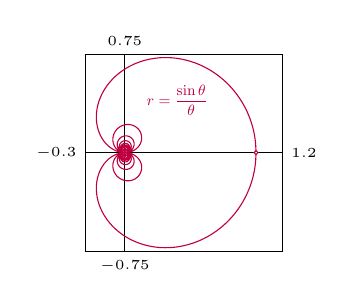
\begin{tikzpicture}[>=latex,xscale=0.25*10/1.5, yscale=0.25*10/1.5][font=\sf\small]

%\draw[xstep=1cm,ystep=1cm,color=gray!20] (-15, -0.5) grid (15, 1);

\draw[] (-0.3, 0) -- (1.2, 0);
\draw[] (0, -0.75) -- (0, 0.75);

\node[left] at (-0.3, 0) {\tiny$-0.3$};
\node[right] at (1.2, 0) {\tiny$1.2$};
\node[below] at (0, -0.75) {\tiny$-0.75$};
\node[above] at (0, 0.75) {\tiny$0.75$};

\clip[draw] (-0.3, -0.75) rectangle (1.2, 0.75);

\draw[purple, samples=400, smooth, domain=25:0.01, variable=\t]
plot ({(sin(\t r))/(\t)*cos(\t r)}, {(sin(\t r))/(\t)*sin(\t r)})--(1,0);
\draw[purple, samples=400, smooth, domain=-25:-0.01, variable=\t]
plot ({(sin(\t r))/(\t)*cos(\t r)}, {(sin(\t r))/(\t)*sin(\t r)})--(1,0);

\draw[purple, fill] (0,0.02) circle(0.014);
\draw[purple, fill] (0,-0.02) circle(0.014);

\draw[purple, fill=white, xscale=0.3, yscale=0.3] ({1/0.3}, {0/0.3}) circle(0.05);

\node[purple, scale=0.6] at (0.4, 0.4) {$\displaystyle r = \frac{\sin \theta}{\theta}$};

\end{tikzpicture}
\end{document}